\documentclass[letterpaper,12pt]{article}
\usepackage{amsmath}
\usepackage{tikz}
\usepackage{pgf-umlcd}
\renewcommand{\umlfillcolor}{white}
\renewcommand{\umldrawcolor}{black}
\usepackage[margin=1in,letterpaper]{geometry}
\usepackage{cite}
\usepackage[final]{hyperref}
\hypersetup{
	colorlinks=true
	linkcolor=blue,
	citecolor=blue,
	filecolor=magenta,
	urlcolor=blue         
}
\usepackage{blindtext}
\usepackage{listings}
\lstset{
  language=python, frame=single, numbers=left, breaklines=true
}
\usepackage{float}


\begin{document}

\title{Seminar: Advances in Dynamic Algorithms \\ Maximal Independent Sets}
\author{Thilo Leon Fischer}
\date{\today}
\maketitle

\begin{abstract}
\end{abstract}


\section{Introduction}

What is a graph?
What is an IS?
What is a MIS?

What is the dynamic setting?
What update is difficult?

All code and files relevant to this report can be retrieved from github.com/thilofischer/dynamic\_mis.

\section{Algorithms}

In this section several different algorithms will be presented to solve the
MIS problem in a dynamic setting.

\section{Implementation}

The algorithms presented in the previous section were implemented using Python
3.8.2 . To store and perform operations on graphs, the \textit{NetworkX}
package was used.
To perform randomized operations, \textit{numpy.random} was used.

\bigskip

The strategy design pattern was applied to give all implementations a unified
interface. This interface is visualised in the UML diagram that can be seen in
figure \ref{fig:uml}.

%
% explain what each funciton does.
%

\begin{figure}[h]
  \begin{center}
  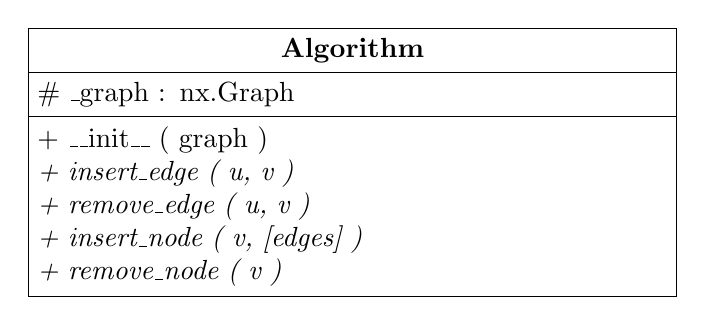
\begin{tikzpicture}
    \begin{class}[text width=8cm]{Algorithm}{0,0}
    \attribute {\# \_graph : nx.Graph}
    \operation {+ \_\_init\_\_ ( graph )}
    \operation [0]{+ insert\_edge ( u, v )}
    \operation [0]{+ remove\_edge ( u, v )}
    \operation [0]{+ insert\_node ( v, [edges] )}
    \operation [0]{+ remove\_node ( v )}
    \end{class}
  \end{tikzpicture}
  \end{center}
  \label{fig:uml}
  \caption{UML Class Diagram of the Algorithm interface}
\end{figure}
% All implementations of a MIS algorithm can share
% To provide a unified interface to all algorithm implementations

\subsection{Testing}
To check that the implementation produces correct results, each algorithm was tested.
The relevant source code is located in the file \textit{tests/test\_algorithm.py}.

To determine whether a set of nodes forms a MIS on a given graph, the function
\textit{Algorithm.is\_valid\_mis()} was implemented.  In the testcases for this
function, an algorithm object was patched using the Python module
\textit{unittest.mock} to return pre-determined values as an answer.
This was done to produce valid and invalid maximal independent sets independently of 
any specific implementation.
The function is tested against four edge cases, three of which expect the
return value to be \textit{false}.

\bigskip

Using the \textit{Algorithm.is\_valid\_mis} function the actual algorithm
implementations are tested.  To generate data for these testcases $G(n,
p)$-graphs were created. To make the testcases reproducible, fixed seeds are
used, so that every run of the testcase operates on the same graph.

For each algorithm four tests are performed.  These testcases correspond to the
four different updates: insert/remove node/edge.  Each testcase consists of a
loop that performs the updates until all nodes/edges are inserted or removed.
For the node insertion case, the starting graph is completely empty. For edge
insertions, the starting graph consists only of nodes.

After each update, it is verified, that the set calculated by the algorithm is
actually a MIS. And that the update has been performed on the graph.  For the
insertion testcases, after all updates have been performed the final graph is
compared against the original graph to check whether the resulting graph is the
desired graph.


\section{Evaluation}

To evaluate the performance of the different algorithms, the execution time of
a set of updates is measured. 
For this purpose five different datasets with varying size are used. 
The datasets are:

\begin{enumerate}
  \itemsep 0em
  \item aves-wildbirds-networks \cite{wildbirds}
  \item topology \cite{konect:2016:topology, konect:zhang05, konect}
  \item facebook-wosn-links \cite{konect:2016:facebook-wosn-links, viswanath09, konect}
  \item youtube-u-growth \cite{konect:2016:youtube-u-growth, konect:mislove2, konect}
  \item brightkite \cite{konect:2016:loc-brightkite_edges, konect:cho2011, konect}
\end{enumerate}

The datasets 1-4 are used for edge insertion benchmarks, while dataset 5 is
used to evaluate edge deletion.

\begin{table}[h]
  \caption{Size of the datasets}
  \label{tab:datasets}
  \centering
  \setlength{\extrarowheight}{0.3em}
  \begin{tabular}{|c|c|c|c|c|c|}
    \hline
    Dataset & 1 & 2 & 3 & 4 & 5 \\
    \hline
    \hline
    Nodes & 202 & 34,761 & 63,731 & 3,223,589 & 52,228 \\
    \hline
    Edges & 11900 & 114,496 & 817,035 & 9,375,374 & 214,078 \\
    \hline
  \end{tabular}
\end{table}

One benchmark run consists of two parts. First
is the initialization of the data structures used by the algorithm. Here, the
initial MIS is calculated for the starting graph, with exception of the
\textbf{ImplicitMIS} algorithm, which does not keep an explicit copy of the
MIS.

The second part of a benchmark run is a loop that calls an \textit{Algorithm} function
to perform an update. In listing \ref{lst:bench}, a slightly modified snippet is shown.

\begin{lstlisting}[label={lst:bench}, caption=Benchmark Code Snippet]
def execute():
      algo = algo_cls(graph)
      for e in edges:
          algo.insert_edge(*e)

t = timeit.timeit(execute, number=1)
\end{lstlisting}

In order for the measured execution time to be reliable, five runs of a
benchmark are done.  The results are then averaged. Averaging is chosen over a
boxplot, because the individual times only show very minor deviations.

Note that in listing \ref{lst:bench} on line 6 the number of runs is set to
one. Because the graph is modified during a run, a new graph instance needs to
be used for each run. However the copy operations to create a new graph do not
depend on the algorithm under evaluation. So these operations should not
contribute to the run time of the algorithm, as they would only introduce more
unknown variables.  Instead the \textit{timeit} function only performs one
iteration at a time and the code shown in listing \ref{lst:bench} is executed
five times.


\subsection{Results}

In this subsection, the results of the benchmark runs are presented. 
The benchmarks were executed on an Intel Core i7-1065G7 with 16GB of memory.

\subsubsection{Edge Insertions}

In table \ref{tab:insertion} the average execution times are shown. The values
are the average over five runs in seconds. In case the execution took too long,
the table contains a \textbf{DNF}.
The threshold for this is 2 minutes. This cut-off was chosen to keep the time required
to perform five iterations of each algorithm manageable. One evaluation of the \textit{Youtube}
dataset for the three fastest algorithm takes over 20 minutes.

For the detailed output, including the time of every single run refer to the
files inside the \textbf{log/} folder in the repository.

\begin{table}[H]
  \caption{Time for Edge Insertions}
  \label{tab:insertion}
  \centering
  \setlength{\extrarowheight}{0.3em}
  \begin{tabular}{|c|c|c|c|c|c|}
    \hline
    Data & Trivial & Simple & Incremental & Dynamic & Implicit \\
    \hline
    \hline
    Wildbirds & 1.281 & 0.013 & 0.012 & 0.064 & 0.020 \\
    \hline
    Topology & DNF & 0.430 & 0.504 & 3.205 & 0.696 \\
    \hline
    Facebook & DNF & 2.582 & 2.228 & DNF & 4.042 \\
    \hline
    Youtube & DNF & 67.058 & 60.695 & DNF & 95.488 \\
    \hline
  \end{tabular}
\end{table}

First note the execution times for the \textit{Trivial} algorithm.
It is considerably slower than the other algorithms on the smallest dataset.
And for the next biggest dataset it does not compute the result in 2 minutes.
This clearly demonstrates the need for a dynamic approach to solve the MIS
problem in a setting with many updates.

Now compare the execution times of all algorithms on the \textit{Wildbirds}
dataset. \textit{Simple} is the second fastest after the improved version of it,
the \textit{Improved Incremental} algorithm. It makes a better choice for removing
a node from the MIS for the cost of an additional degree comparison.

The \textit{Dynamic} algorithm presented in \cite{gupta2018simple} performs
worse than the simpler algorithms. Profiling the code did not reveal
any obvious bottlenecks for these algorithms.

However, inspecting the datasets showed, that in the \textit{Youtube} dataset
only six nodes are considered heavy in the full dataset. In the complete graph
of the \textit{Facebook} dataset no nodes are heavy. The same is true for the
\textit{Wildbirds} network. In the \textit{Topology} dataset three nodes are
heavy in the full graph.

Although it is not as severe, the \textit{Implicit} algorithm is also slower.


Thus it is likely that for these specific datasets, the more sophisticated
algorithms can not realize their full potential.
Rather the higher complexity of the code added overhead, that slowed them down.

% Thus it is likely that this difference is caused by the more complicated
% implementation. This factor is not accounted for when considering the asymptotic
% complexity is evaluated.

A case where this became obvious occured during the implementation of the
\textit{ImprovedIncremental} algorithm. It is almost identical to the
\textit{Simple} algorithm. Thus the first implementation used inheritance. This
approach is shown in listing \ref{lst:slowinc}. However the additional
\lstinline[]{if}-statement and function call negated the speed improvement from
differentiating between the lower and higher degree node. The algorithm that is
faster in theory was actually slower in practice.


\begin{lstlisting}[label={lst:slowinc}, caption={Slow implementation}]
class ImprovedIncrementalMIS(SimpleMIS):
  def insert_edge(self, u, v):
    lower_deg, higher_deg = (u, v) if self._graph.degree(u) < self._graph.degree(v) else (v, u)
    SimpleMIS.insert_edge(self, lower_deg, higher_deg)
\end{lstlisting}

Instead it is faster to inline the code from \textit{Simple}. This inlined implementation
was used for the benchmarks.

% Theoretical does not matter as much for fast code
% comparison  between Simple and incremental

\subsubsection{Edge Deletions}

To evaluate the performance of edge deletions, the \textit{Brightkite}
\cite{konect:2016:loc-brightkite_edges, konect:cho2011, konect} dataset is used.

The edges to be removed were chosen randomly but in a reproducible way. So every
benchmark run performs exactly the same operations. The first benchmark removes
1,000 edges, the second 10,000, the third removes 100,000 edges. For edge
deletions, the \textit{Improved Incremental} algorithm is not used, because it
only supports incremental updates. For deletions, it is identical to the
\textit{Simple} algorithm.

\begin{table}[h]
  \caption{Time for Edge Deletions}
  \label{tab:deletion}
  \centering
  \setlength{\extrarowheight}{0.3em}
	\begin{tabular}{|c|c|c|c|c|c|}
		\hline
		Removals & Trivial & Simple & Dynamic & Implicit \\
		\hline
		\hline
		% 1000 & 2.68 & 0.018 & 0.017 & 0.029 \\
		1000 & 77.246 & 0.136 & 0.158 & 0.100 \\ % the initialisation takes 0.153
		\hline
		10,000 & DNF & 0.157 & 0.266 & 0.166 \\
		\hline
		100,000 & DNF & 0.361 & 1.252 & 0.793 \\
		\hline
	\end{tabular}
\end{table}

In this scenario \textit{Trivial} performs even worse than in the insertion
case. While the three more sophisticated approaches are fairly evenly matched
for few updates. When stepping up from 1,000 deletions to 10,000, the execution
time does not increase very much. This is caused by the slow
initialization phase. In the insertion case, the initial graph consists only of
nodes without their edges. So the initialization is basically a loop that
adds all nodes to the MIS, and thus is relatively fast. However, in the deletion
case, the initial graph is the full dataset. As shown in figure
\ref{tab:datasets}, the brightkite dataset has 52,228 nodes and 214,078 edges.

To initialize, \textit{Simple} performs a single execution of the
\textit{Trivial} algorithm. This alone takes ca. 0.140 seconds, 89\% of the
runtime for 10,000 updates.
When only few updates are performed, the \textit{Implicit} algorithm benefits
from the low initialisation overhead.
Again, the \textit{Dynamic} algorithm from \cite{gupta2018simple}, is the slowest.
In theory, the \textit{Dynamic} algorithm is faster by treating nodes
differently based on their degree. However, after performing the benchmark, inspection
showed, that in this dataset no node is considered to be heavy.


% nicht 10mal solange wegen der langen initialization


% \subsection{What I learned}

\section{Conclusions}

\bibliography{report}{}
\bibliographystyle{plain}

\end{document}

